\subsection{Implémentation avec Max for Live}

\begin{comment}
  L'architecture décrite précédemment est présentée comme un paradigme général, on présente ici l'implémentation concrète.
\begin{enumerate}
  \item Outil populaire dans le domaine de l'EDM
  \item Facilité d'utilisation et intégration dans un environnement 
  \item Prototypage aisé dans M4L
  \item Communication entre les entités d'Ableton Live via messages M4L
\end{enumerate}
On pourrait aisément rendre l'usage plus général en codant un couple de VST fonctionnant sur le même principe.
\end{comment}

L'objectif principal de l'implémentation proposée était de pouvoir expérimenter le plus rapidement possible sur les transformations en tant que musicienne. J'utilise la station audionumérique Ableton Live pour composer et produire de la techno et de la trance, et c'est donc naturellement que j'ai choisi Max For Live pour une première implémentation. 

Max For Live est un langage de progammation haut-niveau complètement intégré à Live. On peut aisément communiquer avec les différences instances du logiciel, ce qui permet dans \emph{LiveScaler} à \emph{Conductor} de contrôler les \emph{Instruments} avec une faible latence.

\begin{figure}[htbp]
  \centering
  \begin{subfigure}{0.86\textwidth}
    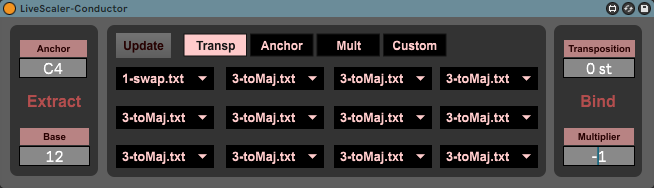
\includegraphics{Figures/LS-Conductor-UI.png}
  \end{subfigure}
  \begin{subfigure}{0.13\textwidth}
    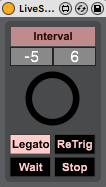
\includegraphics{Figures/LS-Instrument-UI.png}
    
  \end{subfigure}
  \caption{Interface graphique de \emph{LiveScaler} (\emph{Conductor} à gauche et \emph{Instrument} à droite)}
\end{figure}